% Template for a Computer Science Tripos Part II project dissertation
\documentclass[12pt,a4paper,twoside,openright]{report}

\usepackage[indent=0pt,skip=10pt]{parskip}
\usepackage[pdfborder={0 0 0}]{hyperref}    % turns references into hyperlinks
\usepackage[margin=25mm]{geometry}  % adjusts page layout
\usepackage{graphicx}  % allows inclusion of PDF, PNG and JPG images
\usepackage{verbatim}
\usepackage{docmute}   % only needed to allow inclusion of proposal.tex
\usepackage[utf8]{inputenc}
\usepackage{mathtools}
\usepackage{changepage}
\usepackage{url}
\usepackage{blindtext}
\usepackage[dvipsnames]{xcolor}
\usepackage{qtree}
\usepackage{tipa}
\usepackage{dirtree}
\usepackage{svg}
\usepackage[format=hang,labelfont=bf]{caption}
\usepackage{subcaption}
\usepackage[algoruled,vlined]{algorithm2e}
\usepackage{fancyref}

%\raggedbottom                           % try to avoid widows and orphans
\sloppy
\clubpenalty1000%
\widowpenalty1000%

\renewcommand{\baselinestretch}{1.1}    % adjust line spacing to make
                                        % more readable
\newcommand{\vital}{\colorbox{BrickRed}{Vital}}
\newcommand{\veryhard}{\colorbox{BrickRed}{Very Hard}}

\newcommand{\hard}{\colorbox{RedOrange}{Hard}}
\newcommand{\high}{\colorbox{RedOrange}{High}}

\newcommand{\medium}{\colorbox{Dandelion}{Medium}}

\newcommand{\low}{\colorbox{LimeGreen}{Low}}
\newcommand{\easy}{\colorbox{LimeGreen}{Easy}}

\newcommand{\element}{\texttt{Element}}
\newcommand{\pos}{\texttt{Pos}}
\newcommand{\boxT}{\texttt{Box}}
\newcommand{\window}{\texttt{Window}}
\newcommand{\canvas}{\texttt{Canvas}}
\newcommand{\controlbar}{\texttt{ControlBar}}
\newcommand{\timebar}{\texttt{TimeBar}}
\newcommand{\button}{\texttt{Button}}
\newcommand{\playable}{\texttt{Playable}}
\newcommand{\sample}{\texttt{Sample}}
\newcommand{\effect}{\texttt{Effect}}

\newcommand*{\fancyrefalglabelprefix}{alg}

\frefformat{main}{\fancyrefalglabelprefix}{\textbf{algorithm~#1}}
\Frefformat{main}{\fancyrefalglabelprefix}{\textbf{Algorithm~#1}}

\frefformat{main}{\fancyreffiglabelprefix}{\textbf{figure~#1}}
\Frefformat{main}{\fancyreffiglabelprefix}{\textbf{Figure~#1}}

\frefformat{main}{\fancyrefseclabelprefix}{\S~#1}
\Frefformat{main}{\fancyrefseclabelprefix}{\S~#1}

\begin{document}
%TC:ignore
% Change these

\newcommand{\mcandidate}{2416B}
\newcommand{\mfullname}{Jude Howard-Gluckstein Tyrrell}
\newcommand{\mcollege}{Homerton College}
\newcommand{\mtitle}{Notation for Phonological Audio Composition}
\newcommand{\mexamination}{Computer Science Tripos -- Part II}
\newcommand{\mdate}{May 2023}
\newcommand{\moriginator}{Prof. Alan Blackwell}
\newcommand{\msupervisor}{Prof. Alan Blackwell}
\newcommand{\mwordcount}{10814}
\newcommand{\mlinecount}{0}
% Consent to the dissertation made available to University members
\newcommand{\mconsent}{I am content for my dissertation to be made available to the students and staff of the University.}
% For the Declaration of originality
\newcommand{\msignature}{Jude Tyrrell}


\bibliographystyle{plain}


%%%%%%%%%%%%%%%%%%%%%%%%%%%%%%%%%%%%%%%%%%%%%%%%%%%%%%%%%%%%%%%%%%%%%%%%
% Title


\thispagestyle{empty}

\rightline{\LARGE \textbf{\mfullname}}

\vspace*{60mm}
\begin{center}
\Huge
\textbf{\mtitle} \\[5mm]
\mexamination \\[5mm]
\mcollege \\[5mm]
\mdate  % today's date
\end{center}

%%%%%%%%%%%%%%%%%%%%%%%%%%%%%%%%%%%%%%%%%%%%%%%%%%%%%%%%%%%%%%%%%%%%%%%%%%%%%%
% Proforma, table of contents and list of figures

\pagestyle{plain}

\newpage
\newpage
\section*{Declaration of originality}

I, \mfullname{} of \mcollege, being a candidate for Part II of the Computer Science Tripos, hereby declare that this dissertation and the work described in it are my own work, unaided except as may be specified below, and that the dissertation does not contain material that has already been used to any substantial extent for a comparable purpose. \mconsent

\bigskip
\leftline{Signed \msignature}
\bigskip
\leftline{Date \today}

\chapter*{Proforma}

{\large
\begin{tabular}{ll}
Candidate Number:   & \bf \mcandidate                   \\
Project Title:      & \bf \mtitle                       \\
Examination:        & \bf \mexamination, \mdate         \\
Word Count:         & \bf \mwordcount\footnotemark[1]   \\
Code Line Count:    & \bf \mlinecount                   \\
Project Originator: & \bf \moriginator                  \\
Supervisor:         & \bf \msupervisor                  \\ 
\end{tabular}
}
\footnotetext[1]{This word count was computed
by 
}
\stepcounter{footnote}


\section*{Original Aims of the Project}
% At most 100 words




\section*{Work Completed}
% At most 100 words


\section*{Special Difficulties}
% At most 100 words


\newpage

\tableofcontents

\listoffigures

\newpage
\section*{Acknowledgements}


%%%%%%%%%%%%%%%%%%%%%%%%%%%%%%%%%%%%%%%%%%%%%%%%%%%%%%%%%%%%%%%%%%%%%%%
% now for the chapters

\pagestyle{headings}

%TC:endignore
\chapter{Introduction}
\textit{
Since the development of electronic devices, people have utilised them extensively in the creation of art, especially music. From the theremin to synthesizers to trackers and modern day Digital Audio Workstations (hereafter referred to as DAWs), electronics have enabled people to compose music easier than ever before, and to achieve previously unachievable sounds.
}

This dissertation explores the full capability of modern computers to facilitate particular styles of artistic audio composition. It presents a novel piece of software (tuPAC: Totally Usable Phonological Audio Composer) that (achieves) this goal through a graphical user interface, as evaluated against an industry-standard audio composition tool (elaborate on results), and acts as a notation for these compositions.
 
 The research and development in this project was done with guidance from an artist who is interested in composing music with only vocal sounds, experimenting with the structure of spoken language and the sounds made when speaking in order to create art. For the rest of the dissertation, this will be referred to as phonological composition, as it focuses on the manipulation of the structure of language to create an effect, rather than traditional melodic or rhythmic patterns, although these features may also be incorporated into the music. Note that this is not an established term but one that I am using as it best describes the type of composition that the project caters to, but there exists a history of composition styles which fall under this category throughout Western classical and contemporary music.

\section{Artistic Background}
It is useful to see some historical styles of composition which utilise phonological materials, in order to see the form that these compositions might take. This allows us to build an idea of what structural features may be present in a phonological composition and what artists may want to achieve.

The isorhythmic motet is a particular style of polyphonic vocal composition which first appeared in 13th century French music \cite{Bent01}, notably used in the work of Machaut. Polyphonic vocal compositions consist of multiple voices singing different melodies. The defining feature of isorhythmic motets is the repetition and augmentation of rhythmic and melodic patterns - referred to in literature as \textit{color} and \textit{talea} - performed as layered vocals. This style is an early example of music which uses structures which are the focus of this dissertation: layering, repetition and augmentation in vocal compositions.

Steve Reich is a prominent contemporary composer most well known for his work in composing minimalist music. His composition Proverb contains 6 voices which recite a short piece of text from Ludwig Wittgenstein \cite{ReichProverb}. It draws from the medieval polyphonic compositions in style, and repeats and augments the quote throughout the piece. Reich splits up a sentence into smaller parts and repeats these parts individually. In another contemporary composition, O King by Luciano Berio, individual syllables of Martin Luther King's name are pronounced and repeated by a voice throughout the piece. In both of these contemporary compositions, the structure of spoken language is broken down and manipulated by the artist.

\section{Motivation}
 The most popular method of modern digital music production is certainly the DAW. Popular DAWs like Ableton, FL Studio and Logic Pro are used almost universally in the composition of modern music, and such are a go-to for artists looking to create music through digital means.

 However, as we will see in the preparation chapter, the design of these programs doesn't lend itself to all forms of composition equally, and whilst they work well in general, there certainly is different approaches to software design that would better cater to the needs, in terms of ease of use and efficiency, of specific use cases.


\section{Project summary}
In this project, I:
\begin{enumerate}
    \item Develop a computational model that accurately represents the structures of phonological composition.
    \item Create a text-based tool which demonstrates the essential ideas of the model.
    \item Design a user interface which creates a visual representation of this model.
    \item Implement this interface into software, providing a digital audio composition tool for artists as an alternative to existing tools, supporting a different approach to composition.
\end{enumerate}

Each of these goals were successfully completed and this dissertation presents the results, as evaluated using standard human-computer interaction techniques.

\chapter{Preparation}
This chapter describes the research and preparation that was necessary before the implementation of the text-based and graphical tools. First, we look at what was needed for this project to succeed.

\section{Requirements Analysis}
In the project proposal, four success criteria were set out for this project. Here, these criteria are broken down and realised into specific achievable tasks, along with some additional possible extension tasks.

\begin{table}[h]
    \centering
    \begin{tabular}{|c|c|c|}
        \hline
         Task & Priority & Difficulty \\
         \hline
         Develop model of composition & \vital & \medium \\
         \hline
         \multicolumn{3}{|c|}{Text-based tool capabilities} \\
         \hline
         Play audio & \vital & \easy \\
         Represent model & \vital & \medium \\
         Apply effects to audio & \medium & \easy \\
         Mapping IPA characters to samples & \medium & \easy \\
         Render sounds as spectrogram & \low & \veryhard \\
         \hline
         \multicolumn{3}{|c|}{Graphical tool capabilites} \\
         \hline
         Build responsive GUI & \vital & \medium \\
         Play audio loaded from file & \vital & \medium \\
         Represent model & \high & \hard \\
         Ensure time keeping of audio & \high & \hard \\
         Apply effects to audio & \medium & \medium \\
         Adjust playback speed for audio & \medium & \hard \\
         Neural synthesis integration & \low & \veryhard \\
         \hline
    \end{tabular}
    \caption{Table of possible tasks to be completed.}
    \label{tab:req_anal}
\end{table}

Whilst some the above tasks are necessary for the project's success, the true success of the project will come from the clarity, usability and efficiency of the interface, for actual users. This success cannot be measured just by the functionality and design choices of the interface, but through user testing, as was carried out in the evaluation stage of the project.  The evaluation measures the projects success in terms of:
\begin{itemize}
    \item Usability: The ability for the program to make the user's life easier by making common actions fast and intuitive.
    \item Clarity: There is a clear correspondence between what happens on the screen, and what the user imagines is happening to their composition. When the user makes a change, the program changes the audio appropriately, how the user expects.
    \item Functionality: The user is not limited in what they are able to do, and can achieve whatever they want to do with the program.
\end{itemize}

\section{Existing Tools}
Studying existing designs of similar software provides reference for what people will generally expect from audio production software, as well as highlighting areas where traditional designs fail in facilitating unconventional styles of composition. This is imperative for the design of this project to improve upon what exists already.

\subsection{Digital Audio Workstations}
In this dissertation, I will primarily focus on Ableton Live when discussing DAWs, as it is the one I personally have the most experience with and it is commonly used in electronic music production. It is also the DAW used for evaluation against my project.

\begin{figure}[h]
    \centering
    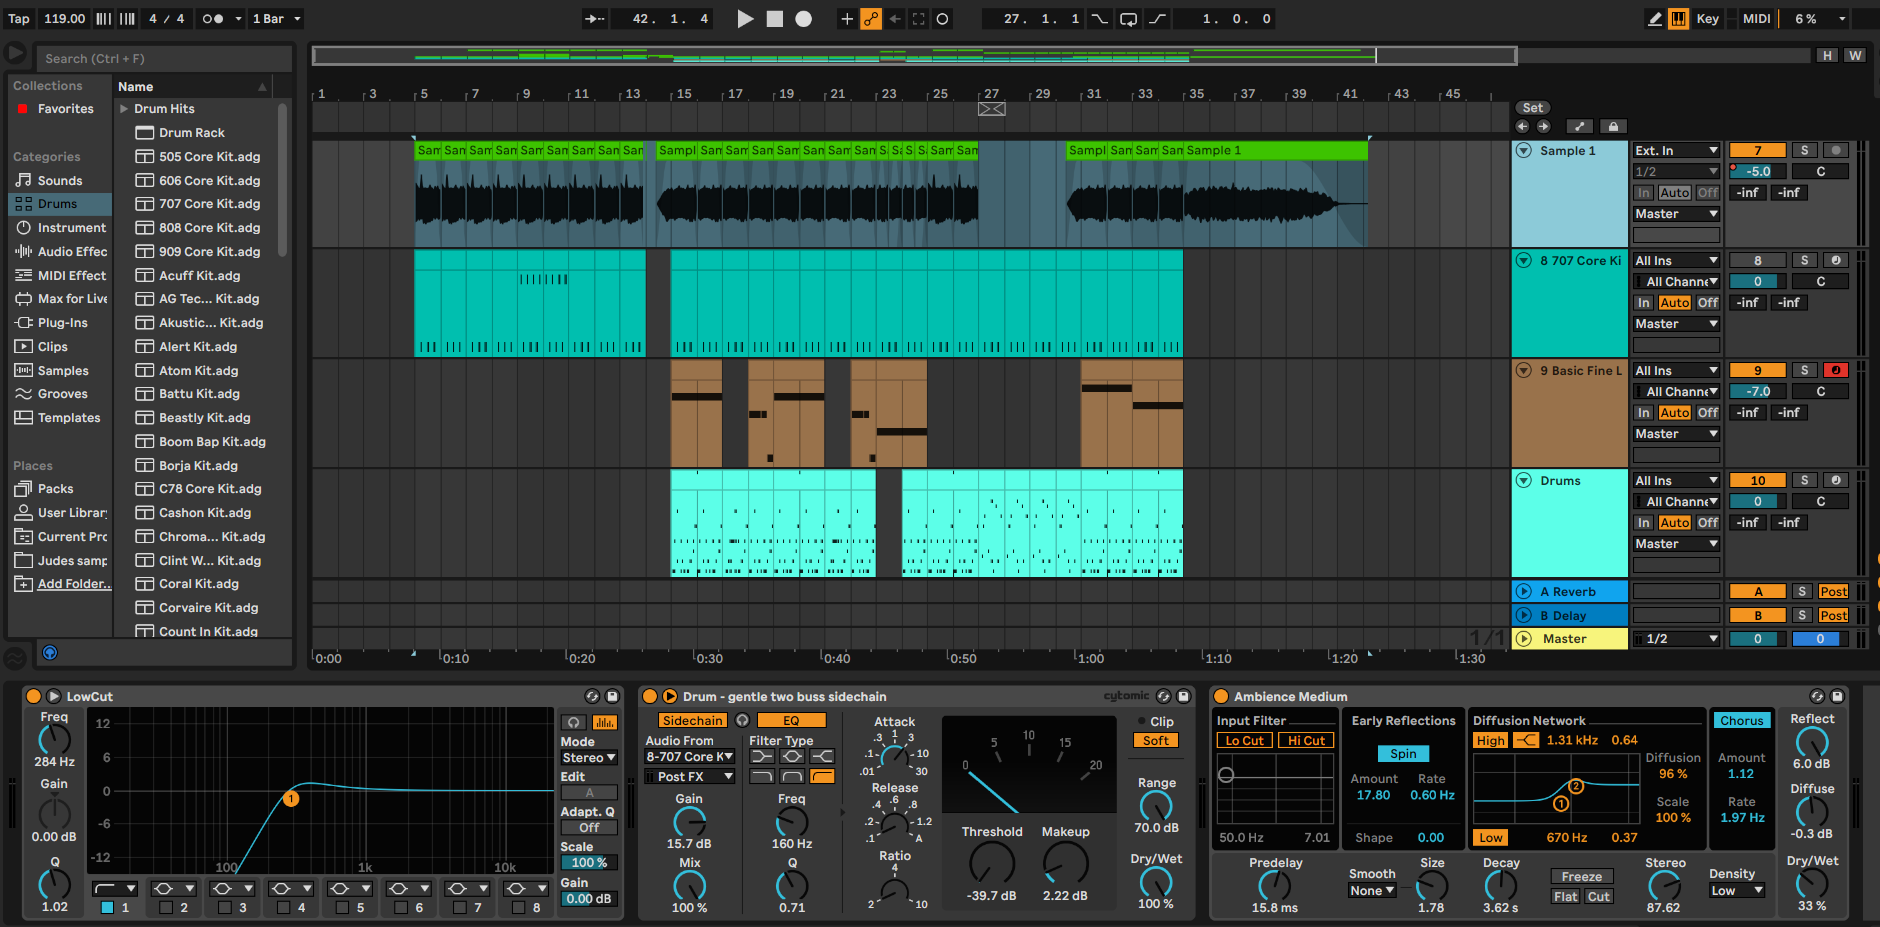
\includegraphics[scale=0.3]{images/ableton example.png}
    \caption{UI of Ableton Live}
    \label{fig:ableton}
\end{figure}

Ableton Live's main interface consists of ``tracks" which can contain either sound clips or MIDI sequences which define the pitches and timing of notes to be digitally generated. The horizontal axis represents time, starting from the left and moving to the right, and the vertical axis generally represents different instruments (separate trakcs), and sometimes pitch. Effects can be added to and parameters adjusted on individual tracks or groups of tracks. 

This structure and design, typical for DAWs, works with an intuition that lines up with traditional composition - each track corresponds to an instrument which can be fed through different effects. Visually, this approach resembles modern staff notation (see \Fref[main]{fig:staff_not}), where the horizontal axis represents time, vertical axis represents pitch, and different instruments or parts are placed on separate staffs (collections of 5 horizontal lines).

\begin{figure}[h]
    \centering
    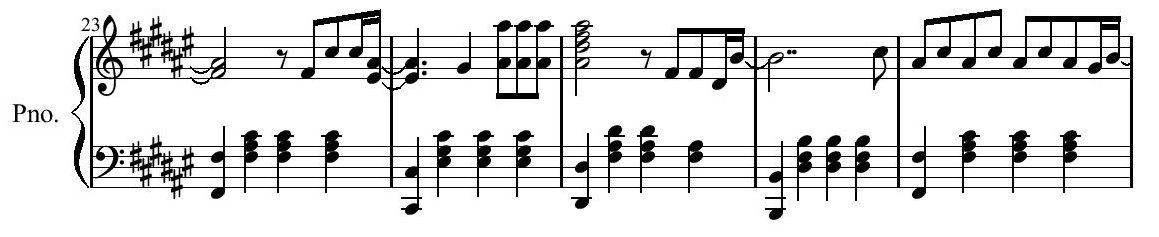
\includegraphics[scale=0.7]{images/modern staff notation.png}
    \caption{Example of modern staff notation}
    \label{fig:staff_not}
\end{figure}

This representation of audio is clearly established and will have been encountered by almost all musicians. This is important as users will expect certain features implicitly from all designs, such as the horizontal axis representing the passing of time from left to right.

Whilst this typical representation has been refined for centuries and proven to be efficient for expressing the intentions of Western classical composers, particularly when composing for standard ensembles of instruments like orchestras, there is many styles that don't fit as well into this notation. This can be observed in the notation for Joshua Alvarez Mastel's composition ``animal"\footnote{\url{https://joshuamastel.com/animal/}}, which has an extremely complex, difficult to understand score. This piece was given as an example by the artist involved with this project as an exemplar phonological composition.

\subsection{Live Coding}
An extisting alternative to DAWs for digital composition is live coding, a technique used to generate art in real time using a programming language. For music, a popular example is Sonic Pi.

\begin{figure}[h]
    \centering
    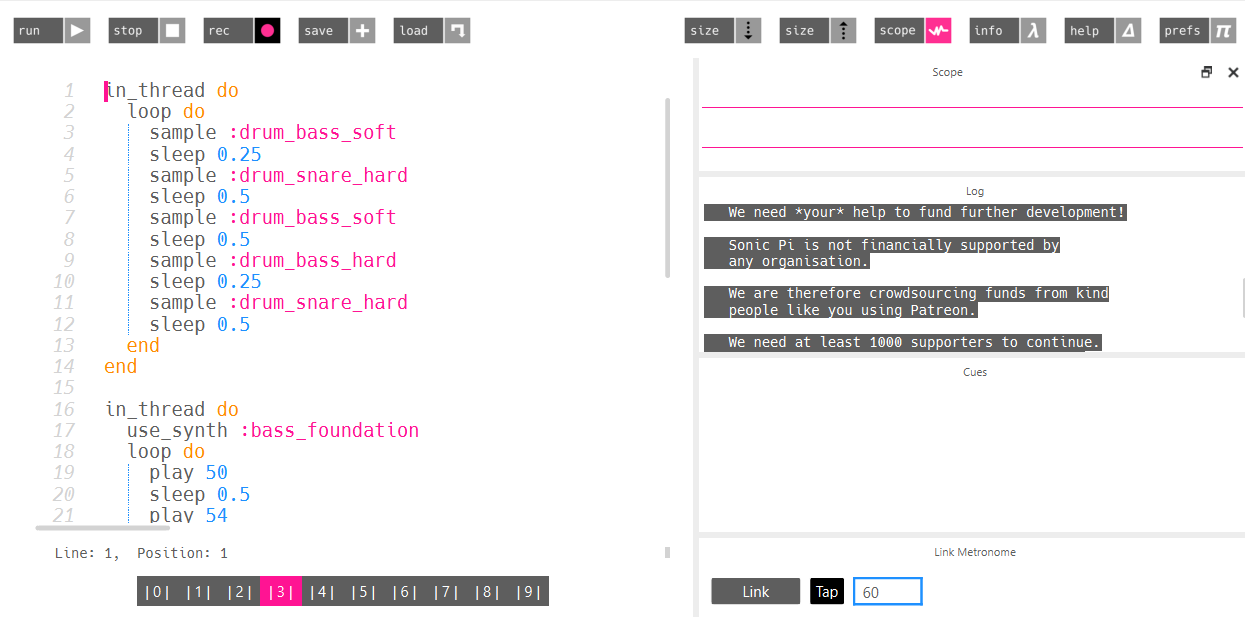
\includegraphics[scale=0.4]{images/sonicpi.png}
    \caption{UI of Sonic Pi}
    \label{fig:sonic_pi}
\end{figure}

Live coding software allows users to generate audio through writing programs, with the defining feature being the ability to modify the code whilst the audio is running and seamlessly change the audio as it is played. This approach to making music is vastly different from industry-standard DAWs, and is often used for performance art.

Live coding platforms differ from DAWs in that there is generally less complex functionality, with more focus on simpler but easier manipulation, particularly the repetition and augmentation of sounds previously defined. This makes the process of live coding plausible in real time whilst still sounding good. This approach is much closer to the goal of this project, and so was a primary focus of research and preparation.

The design of live coding platforms is highly related to this project, as they focus on defining sounds and loops of sounds which are played back live, and augmented as they play. However, live coding platforms, being text-based, have no graphical interface and so are inaccessible to artists who are less tech-savvy and also provide no visual notation for the music being composed.

\section{Sonic Pi and Strudel}
In preparation for the development of the project, I researched two live coding platforms in order to build my text tool using the framework of one of them.

Sonic Pi is written in C++ and Ruby. The GUI is written in C++ whilst the code parsing and audio generation is done in Ruby. It synthesises audio by sending OSC (Open Sound Control) messages to SuperCollider, which keeps track of all synthesisers, samples and effects being triggered by the Sonic Pi interface. The codebase is large but it has an API meaning that one could develop their own platform and use the Ruby portion of the software to generate sound using SuperCollider easily without the C++ GUI.

Strudel is a web-based live coding platform built in Javascript, based on another live coding language called TidalCycles. It mainly uses the Web Audio through a framework called Tone.js to synthesise audio, and was still in an experimental stage of development at the time of this project being researched. The software is relatively small, and the codebase easy to navigate and manipulate, as it is written in a modular style that splits up different parts of the software into separate packages which can be used individually.

I decided to continue my research using the Sonic Pi platform, as Strudel is too incomplete in its current form to work with and could cause additional difficulties down the line.

\section{Speech synthesis}
Whilst preparing for the project, it was unclear exactly what the functionality of the tool would include. An obvious idea was to include a way of generating phonological sounds digitally, to allow the user to utilise and manipulate speech sounds without recording and re-recording themselves speaking. However, digital speech synthesis is an extremely difficult task and was largely ruled to be out of scope for this project. It is possible to generate very basic vowel sounds without too much difficulty, but producing parameters which are able to be manipulated in a way that makes sense intuitively is almost impossible. I experimented with vowel synthesis during the implementation of the text tool, as will be detailed later.

\section{Software Engineering}
In preparation for the implementation of this project, research was conducted to decide the specific tools and techniques that would be used. It was necessary to find what approach would allow for the project to be implemented fully, but not require excess development time. Some of that research, and the final decisions for implementation, is outlined here.

\subsection{Framework}
As mentioned, Sonic Pi was used to develop the text tool as it provided the necessary features for its demonstrative purposes.

For the graphical interface, I needed a platform that was as powerful as possible to support my development, but malleable enough to accurately represent the design of the tool. I also needed something that would be capable of generating the audio well, through a powerful library or easily connecting to other software.

Qt is a C++ framework of libraries which facilitates the development of powerful desktop applications, with a powerful GUI library. It was used to build Ableton, Sibelius and MuseScore, which are three of the most popular musical composition tools on the market. However, this complexity would make it too cumbersome to work with for the scope of this project.

Electron is a Javascript framework which builds desktop applications using Chromium, rendering a web-page in a native window. This makes it relatively easy to use and inherently cross-platform, although that isn't of much importance for this project. It uses Node.js for Javascript. Node.js is convenient and enables the use of essentially any Javascript library, through the npm package manager. Electron is a popular, well-documented framework, which is beneficial in a project with little development time. It powers applications like Discord, Skype, Twitch and Notion.

After researching various options, I decided to work with Electron for its ease of use considering the limited development time of this project.

\subsection{Libraries}
\subsubsection{Audio}
I considered using SuperCollider directly with my project, but eventually decided not to. SuperCollider is extremely powerful, but could have cause a lot of implementation issues due to its complexity. There is a library available for Javascript named supercollider.js, but even with this library, the complexity of SuperCollider would be a considerable difficulty in the implementation of my tool, and the added functionality and modularity over simpler audio libraries is not necessary for my project.

Tone.js is a Web Audio framework which supplies an API for audio applications written in Javascript. It supplies reliable event scheduling, audio playback from files and a system for linking effects and sounds together, and through to output. The features supplied by this library are sufficient for this project, and should be easy to implement, so was chosen for the time-keeping and audio playback of the graphical tool. It is also used in Strudel as one of the main options for audio generation. Based on the ease of implementation, and established widespread usage, this library was chosen for my project.

\subsubsection{Visual Interface}
p5.js is a Javascript library which provides basic graphical capabilites, with a co-ordinate system. It is easy to use, and doesn't have a lot of overhead, which allows for the developer to have full control over what is rendered in the application. Because of its fluidity, it was chosen as the library for this project.

\subsection{Programming Languages}
The text tool was written in the Sonic Pi GUI, in Sonic Pi's own language, which is essentially Ruby.

After research into both Javascript and Typescript, it was decided to write the project in Typescript, which is an extension of the Javascript language which allows static type checking, and transpiles into Javascript code. It also adds a few features that make object oriented programming easier, which was deemed valuable to the project.

\subsection{Development Methodology}
It is important to approach software development with a solid plan and logical steps from beginning to conclusion. Due to the experimental nature of this project, it was impossible to know exactly how the implementation would go from start to finish, and so it took part in two stages. 

The first stage would consist of the development of the text-based tool and the computational model of composition. This stage used iterative development, taking advantage of the ease of implementation of features in Sonic Pi to supply the artist involved with regular updates, getting feedback on what is useful for the artist and what isn't as necessary and wouldn't be a priority in the graphical tool. This would refine the idea of what is crucial to the structure of phonological composition being represented in a graphical interface.

The second stage would consist of the development of the graphical tool, which suits the waterfall development methodology. At this stage, the graphical tool would be fully planned out and designed, and so the development could be broken down into the implementation of individual features, with essential prerequisites like playback of audio being fully implemented before features that need others to be implemented, like audio effects.

\subsection{Tools}
For the development of the text-based tool, I simply used Sonic Pi's GUI to write code.

For the graphical tool, I used Visual Studio Code as an IDE. VS Code was an obvious choice, as it is powerful and very customisable. There exists many community made extensions which can enable one to use various tools easily with your code, such as better support for TypeScript. It has a built-in Git tool which made for easy version control and backing up.

I used GitHub to backup my repository and Git for version control. As stated, this was easy to do with VS Code. This minimised the risk of data loss, as even if my laptop was lost or destroyed, I could retrieve my work. In the same vein, I wrote all of my notes during the project in Notion which automatically backs everything up to the cloud.

\section{Starting Point}
Here, I declare the previous knowledge and skills that I did and didn't have prior to the implementation of the project.

In Part IB, I took the Formal Models of Language course, and in Part II, I took the Natural Language Processing unit of assessment. These courses provided me with insight into the structure of language which is discussed in the implementation and was relevant to the development of the project.

\subsection{Text tool}
The text tool was built in Sonic Pi's own language, which handles everything from audio generation to time keeping. As the text tool was only for demonstration to the user and exploration of possible useful features, this was sufficient. I have only briefly used Sonic Pi prior to this project and was required to learn its native language, which is based on the programming language Ruby, which I have also never used before.

\subsection{Graphical tool}
The graphical tool for the project was built using Electron and Node.js, and written in Typescript. The sound was generated using the Tone.js library, which has a reliable time-keeping system. I have never used Javascript, Typescript, Electron, Node.js or Tone.js in any previous work. I have previously used the Python version of p5.js, Processing, which is very similar to the Javascript library.

\chapter{Implementation}
This chapter outlines how both the text-based tool and the final graphical tool were designed and implemented.

\section{Text-based tool}
As described in the preparation, it was decided that Sonic Pi had all audio functionality necessary to experiment with possible features that would benefit phonological composition, and to get feedback from the artist.
\subsection{Phonological composition structure}
\textit{Note: here I am primarily talking about English, as it is the only language I know. Much of the analysis applies directly to other languages, but certain concepts such as morphemes and syllables are subtley different across the world.}

In order to develop the text-based tool, it is important to first understand what the compositions might look like and so an understanding of phonological structures is vital. In linguistics, it is common to represent language as a tree, with individual words as leaf nodes. 
\begin{figure}[h]
    \centering
    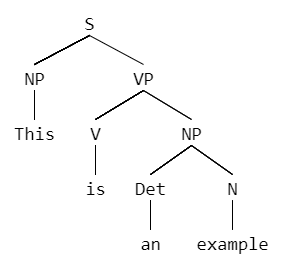
\includegraphics[scale=0.5]{images/parse_tree.png}
    \caption{An example of a grammatical parse tree}
    \label{fig:parse_tree}
\end{figure}

The tree structure is used as it accurately represents the structure of many written natural (as well as formal) languages, like English. A key feature of the tree structure is the idea of recursion; a node in a tree can contain nodes with the same structure as itself, continuing on indefinitely. Interestingly, in a seminal article from 2002, M. Hauser, N. Chomsky and W. Fitch argue that recursion is the singular feature of that distinguishes the human faculty of language from other animals \cite{Hauser02}. In these trees, words are the smallest possible units of language, but in alphabetic languages, words are made of morphemes, which in turn consist of one or more letters. This idea of breaking up sentences, phrases and words into smaller pieces is of particular interest for phonological composition, as seen in the preparation chapter.

This analysis motivates the necessity for a recursive structure in the design of the tools. There needs to be a concept of elements containing smaller elements which could contain smaller elements still, until we get down to individual spoken sounds.

In spoken language, this structure persists still, but words are represented through sound. These sounds can be characterised as individual syllables, or in writing by a phonetic notation, such as the International Phonetic Alphabet (IPA), which was of interest for this project.
\begin{figure}[h]
    \centering
    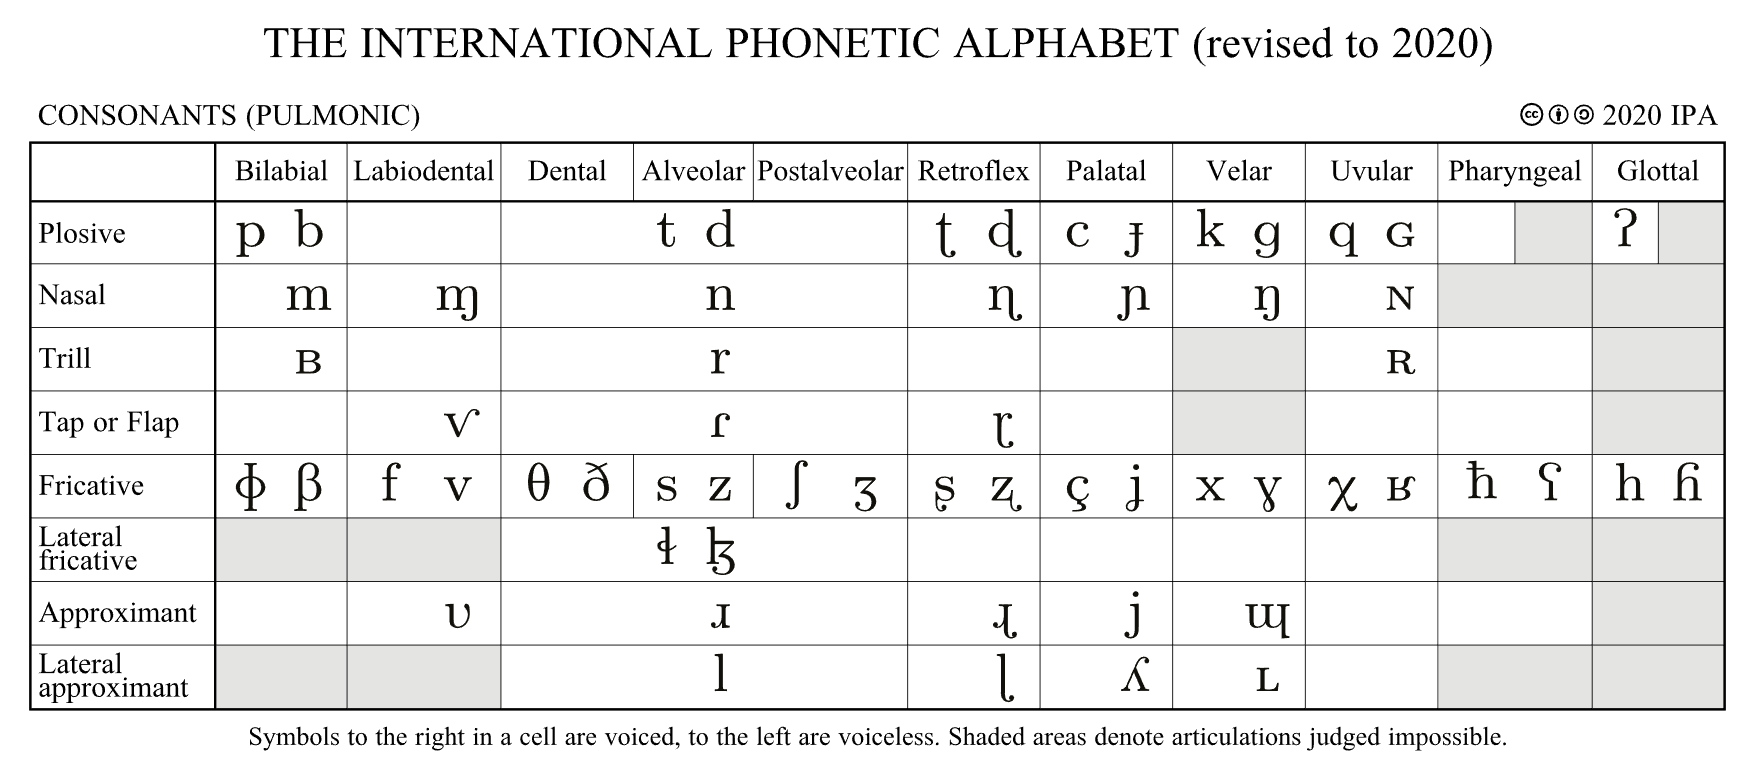
\includegraphics[scale=0.3]{images/IPA.png}
    \caption{A portion of the official IPA chart.\protect\footnotemark}
    \label{fig:ipa_chart}
\end{figure}
\footnotetext{Image from International Phonetic Association, under the CC BY-SA 3.0 license: \url{https://creativecommons.org/licenses/by-sa/3.0/deed.en}, cropped by myself}

An idea for the text tool was to represent sounds by characters from the International Phonetic Alphabet, as they cover almost all sounds used in human spoken language. Characters in the IPA represent vocal sounds or modifications to vocal sounds which have a lexical impact on what is being said. That is, if you were to replace one sound or modification with another, the meaning of the word being said may change. It was discovered during research that there is no problem using IPA characters in Sonic Pi, and they can be used in strings and even as function and variable names.

The letters in IPA represent consonant or vowel sounds, which can then be modified by diacritics. For example, the character b represents the first sound in the English word ``bit", and we can attach a diacritic to have it read in ``breathy voiced" form: \textsubumlaut{b}.

With this in mind, we have two elements for the design. The narrative structure of the composition, which relates to the linguistic tree structure, and the actual sounds and modifications to sounds being made.

\subsection{Vowel synthesis}
FIX THIS SECTION - MORE TECHNICAL DESCRIPTIONS ALL OVER


Whilst it was clear general speech synthesis was never going to work, there was some exploration into audio synthesis mimicking vowel sounds. By generating a sawtooth wave, applying a bandpass filter and some other effects, you can make decent vowel sounds. All of these features are present in Sonic Pi, so I decided to experiment with it.

In the end, I scrapped this as it didn't sound good enough to incorporate into the project and to expend development time on, so for the rest of the project I focused solely on using samples in my tools.

\subsection{Computational representation}\label{sec:comp_rep}
In order to represent this structure, it is clear we want to organise sounds recursively, so we can define a word as a collection of syllables, or a line as a collection of words. There is a number of ways to achieve this computationally.

A natural approach would be object oriented programming. Defining a type which could either contain a sound clip or a collection of objects with the same type supplies all the capability needed to represent the aforementioned phonological tree structure. Objects which simply contain a sound clip are leaf nodes in the tree and objects containing collections of other sound objects are the parent nodes. These nodes could have names denoting what structure they represent, such as a syllable, word or sentence.

\begin{figure}[h!]
    \centering
    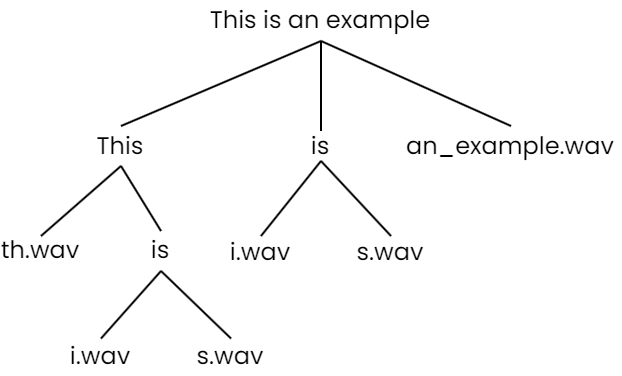
\includegraphics[scale=0.5]{images/tree_structure_example.png}
    \caption{Example of a possible structure with this approach}
    \label{fig:tree_struct_ex}
\end{figure}

Unfortunately, Sonic Pi does not allow for classes to be created so this approach does not apply for the text tool. Instead of dedicating a class to each of these objects, we could instead use lists which either contain more lists or sound files, as previously described. This was the approach I ended up using for the text-based tool.

It is still desirable to have parameters set on the sounds, though, even without being able to define a class which would have these parameters as its local fields. For this, we could store the sound files as a tuple, containing a file name referring to a sound file to be played, along with one or two parameters.

\subsection{Final text-based tool}
The final implementation of the text-based tool consists of a collection of functions which can:
\begin{itemize}
    \item Create lists of sounds.
    \item Translate a string of IPA characters into a list of file names storing the sounds they represented.
    \item Take a list containing sounds, or other lists, and play them back with the appropriate timing.
    \item Reverse a list of sounds (in a deep sense, each list contained in the list would also be reversed).
    \item Set all sounds in a list to last the same duration.
\end{itemize}

Sounds are represented by a tuple:
\begin{equation*}
    \{sample,\ length,\ gap\}
\end{equation*}

sample - Stores a string referring to a file name, to be played.

length - The amount of time the sample should play for, relative to how long the sample is. The sample is stretched such that it is played for $sample_duration * length$ seconds.

gap - The amount of time after the sound plays that the next sound should start, relative to the duration of the sample. After playing this sound, the program waits $sample\_duration * length * (1 + gap)$ seconds before playing the next sound. If this value is negative, the next sound will overlap with the current sound, which can make for more realistic speech when using individual consonant/vowel sounds.
\newpage
\section{tuPAC}

This section describes the culmination of all previous work described in this dissertation, the design and implementation of the Totally Usable Phonological Audio Composer, or tuPAC for short.

\subsection{Visualising compositional structure}
When designing the graphical interface, it is vital to have an accurate visual representation of phonological composition, in order for the user to easily create and manipulate them whilst using it. There needs to be a clear representation of individual sounds, and the components containing those sounds. I looked at the design of other software for inspiration.

\subsubsection{Scratch}
Scratch is a very popular visual programming language that is commonly used to introduce children to the ideas behind programming without the difficulty of writing code in a text form, which can be intimidating at first. This platform was in my mind from the beginning of the project because of the similarity in motivation with my program, making a visual interface to improve accessibility to a task which is typically complex and technically done digitally. 

Scratch uses blocks to represent events in either the project or the control flow of the events. These blocks are dragged over from a menu and put arranged how the user desires on a blank surface.

\subsubsection{Field}
A major source of inspiration for the program's final interface was Field, which is a live coding software made by OpenEndedGroup\footnote{Github repository of Field: \url{https://github.com/OpenEndedGroup/Field2}} not for music, but for visual art. The live coding background means that this design is very relevant to my own project. The interface consists of a canvas which can contain boxes, which can have code written to be associated with them. A line marking the current ``time" runs over the screen, executing code in boxes as the line runs over them. The code can use the current position of the line as a parameter, and the code is used to generate visuals. Field allows users to generate moving digital art.

WRITE MORE HERE

\newpage
\subsection{Final Design}
\begin{figure}[h]
    \centering
    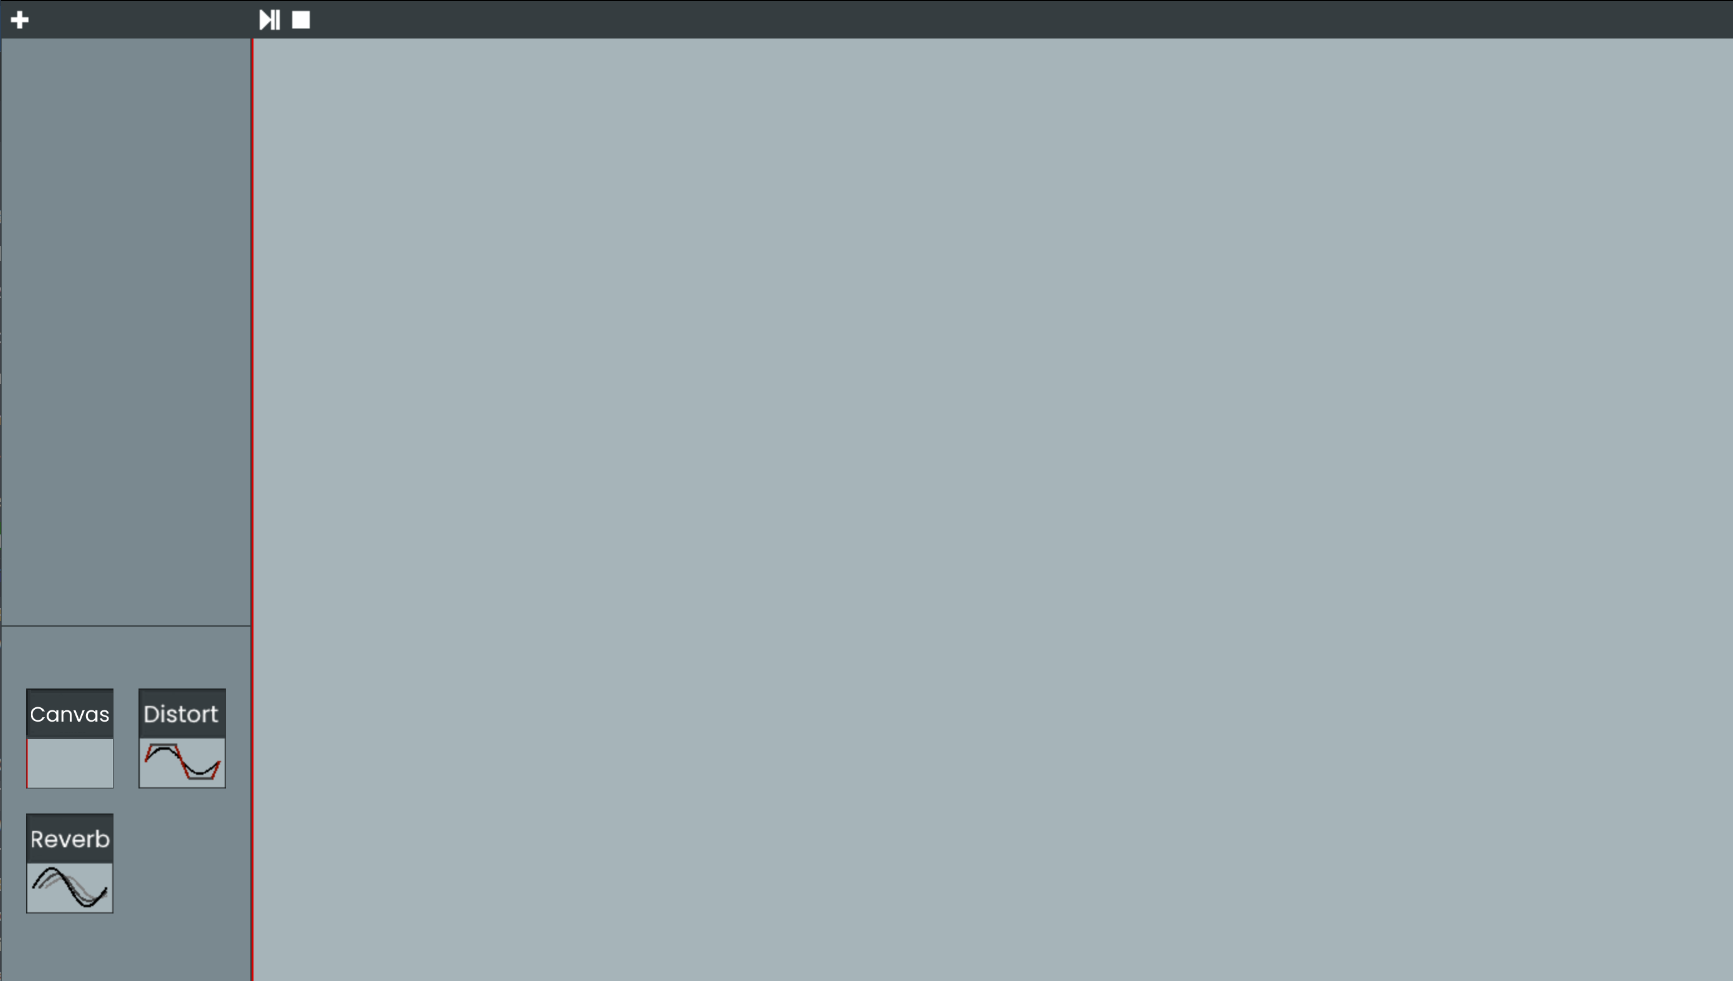
\includegraphics[scale=0.4]{images/tuPAC_GUI.png}
    \caption{The GUI of tuPAC}
    \label{fig:tupac_gui}
\end{figure}
RE-WRITE/SCRAP?

The final design incorporates ideas from Field and Scratch and creates a visual representation of the phonological composition structure. The interface consists of a main canvas, an element menu, and a file menu. The canvas is much like the canvas in Field, with a line moving from left to right, activating boxes representing sounds as it passes over them. In order to represent the recursive type of the canvas, we have the boxes in the canvas to be either a sample linked to a sound file, or another canvas, with all of the capabilities of the main canvas.

This design was the final step before the implementation of the graphical tool. Next, we will look at how the tool works.

\subsection{Program structure}
Figure \Fref[main]{fig:tupac_structure} gives an overview of the general structure of the software at runtime. The \verb|main.js| file is run first, which imports Electron, which contains Node.js and Chromium. It creates a window with the layout described by \verb|index.html|. On loading the webpage, \verb|tupac.js| is run, creating a p5.js canvas on the page. The p5.js library runs the setup function once and then repeatedly runs the draw function. These functions are defined in \verb|tupac.js|.

\begin{figure}[h]
    \centering
    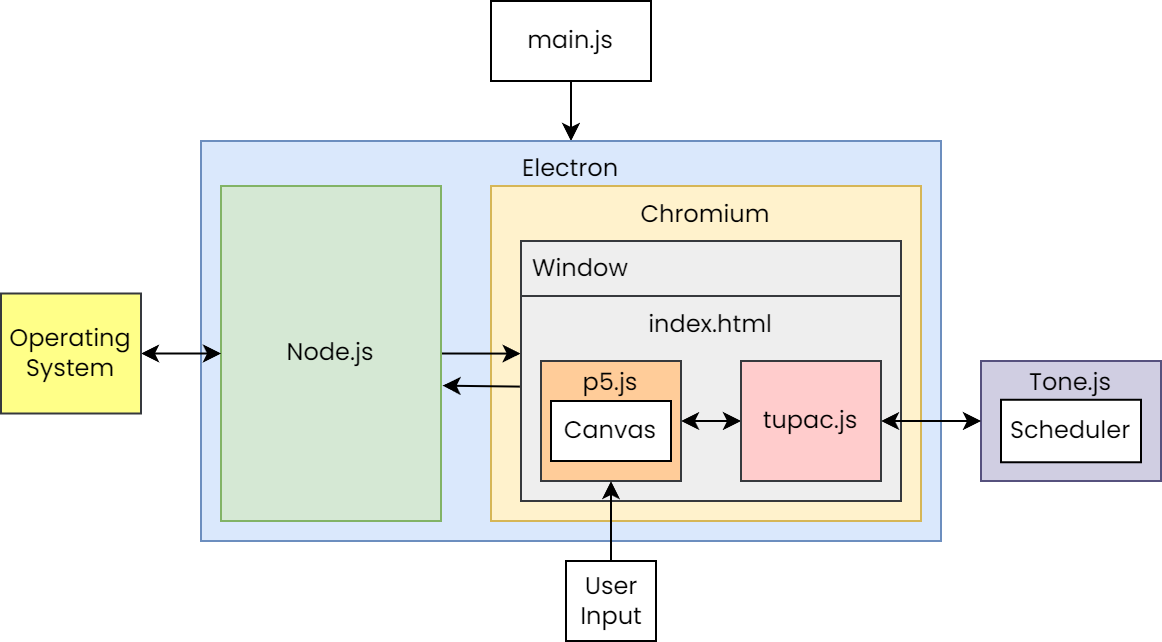
\includegraphics[scale=0.4]{images/tuPAC_structure.png}
    \caption{High-level runtime structure. Arrows indicate some form of communication between parts.}
    \label{fig:tupac_structure}
\end{figure}

As mentioned previously, TypeScript was used in order to support the usage of the object oriented programming paradigm, which reflects the design of this program. We want the ability to instantiate objects of a certain type, and pass objects around knowing they will have certain methods, which isn't possible in vanilla JavaScript as it is dynamically typed. In the \verb|/src/| directory, each file contains one or two classes, which are imported by other files to be used in the running of the program.

When the setup function in \verb|tupac.js| is run, it instantiates a \window\ object, and populates it with the two side menus and a main canvas, as shown in Figure \Fref[main]{fig:tupac_gui}. The rest of the program then relies on user input.

\subsection{Elements}
In tuPAC, everything that is rendered on the screen is an \element, i.e. every class that will be rendered extends the abstract \element\ class. The \element\ class defines the members and methods that everything in the program needs to have, and provides default versions for them.

\begin{table}[h]
    \centering
    \begin{tabular}{c|c|p{300pt}}
        Name & Type & Description \\
        \hline
        pos & \pos & The co-ordinates of the top-left corner of the \element\\
        size & \pos & The size of the \element\\
        minSize & \pos & The minimum size to allow when resizing\\
        draggable & \verb|boolean| & Whether this \element\ can be moved by the user\\ 
        resizable & \verb|Resi| & Whether this \element\ can be resized, in each direction\\
        parent? & \element & The \element\ which contains this one. If this \element\ is on the top level, then this is \verb|null|\\
    \end{tabular}
    \caption{The members defined in the abstract \element\ class}
    \label{tab:element_members}
\end{table}

In Table \Fref[main]{tab:element_members}, \verb|Resi| refers to an Enum\footnote{\url{https://www.typescriptlang.org/docs/handbook/enums.html}} which can be set to any of the values in the set \{None, X, Y, XY\}, indicating whether the \element\ can be resized by the user in the X and Y directions. The \pos\ class is described in section \S\Fref[main]{sec:pos}.

\begin{figure}[h]
    \centering
    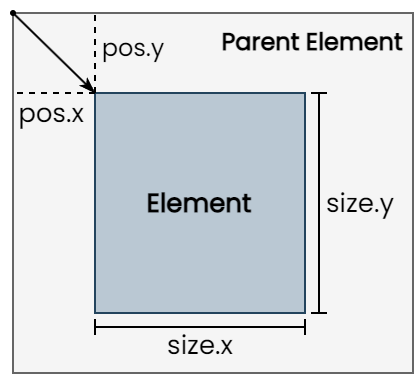
\includegraphics[scale=0.6]{images/element_demonstration.png}
    \caption{The meaning of the size and pos members of \element. If an \element\ has no parent, this refers to the application's window.}
    \label{fig:element_demo}
\end{figure}

The \element\ class supplies a number of methods which are useful for all \element s to have, or can be overridden by sub-classes. Two methods are left abstract, meaning that sub-classes need to have an implementation in their definitions. These methods are \verb|draw| and \verb|clicked| and, as one might guess, are called when the \element\ should be drawn onto the screen and when a user clicks on it, respectively.

Note that the p5.js library uses the top-left corner as the origin of co-ordinates, meaning that the x co-ordinate indicates the distance from the left-hand side of the window, and the y co-ordinate indicates the distance from the top of the window. In tuPAC, this convention is maintained.

\subsection{Instrumental Classes}
\subsubsection{Pos \& Box}\label{sec:pos}
Being a graphical software, tuPAC makes frequent use of co-ordinates and pairs of co-ordinates. The classes \pos\ and \boxT\ help with the handling of these by wrapping these up into single objects and providing methods to easily manipulate them.

\pos\ objects have two members: x and y. The class provides methods such as adding co-ordinates together, multiplication by a scalar and finding the piecewise minimum of two \pos\ objects.

\boxT\ objects have two members: origin and size. These members are both \pos\ objects specifying the position of the top-left corner and size of a box, respectively. This class supplies methods to check whether a co-ordinate is in a \boxT\ and move a \boxT's origin such that it sits inside a larger \boxT, et cetera.

\subsubsection{Control Bar}
Many of the \element s in tuPAC have bars along the top which can be used to drag them, can have buttons which control the \element, and can have text to describe them. These are referred to as \controlbar s, the name of the class which defines these objects.

\subsubsection{Playable}
\playable\ is an interface that specifies \element s that can be played. It ensures that all \playable\ \element s have methods for playing, pausing, stopping and scheduling playback.

\begin{figure}[h]
    \centering
    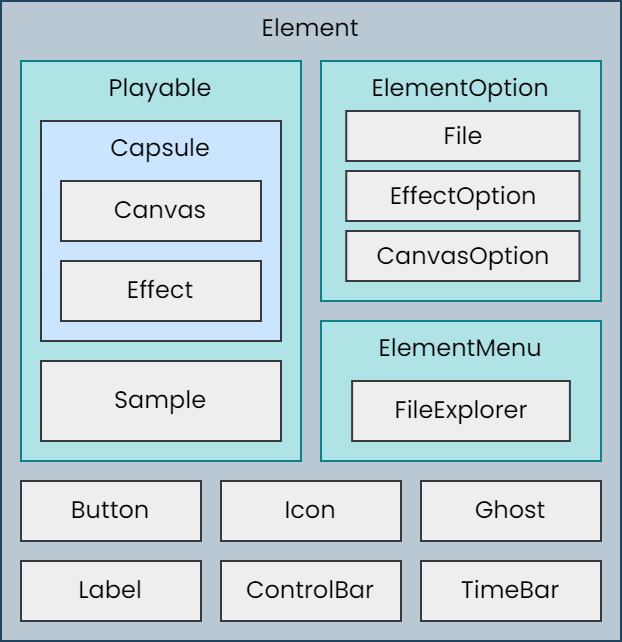
\includegraphics[scale=0.6]{images/tupac_class_structure.png}
    \caption{The inheritance structure of all classes that extend \element. All smaller boxes contained in larger boxes are sub-classes of the larger box.}
    \label{fig:element_inheritance}
\end{figure}

\subsection{Canvas}
The most important \element\ in tuPAC is probably the \canvas. When the program first starts, the user is presented with a blank \canvas\ object, alongside the menus. This class represents the nodes of the phonological tree structure as described in \S\Fref[main]{sec:comp_rep}. They represent a sound or a collection of sounds; when a \canvas\ plays, its \timebar\ moves from left to right, and any sounds underneath the bar get played.

\begin{figure}[h]
    \centering
    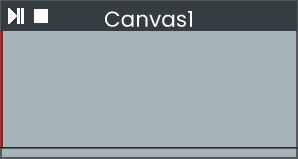
\includegraphics{images/canvas.png}
    \caption{An example of a \canvas.}
    \label{fig:canvas}
\end{figure}

\canvas\ objects consist of:
\begin{itemize}
    \item A \controlbar\ with a title, play/pause button and stop button. The play/pause button starts the \canvas\ playback if it is paused, and pauses the \timebar\ where it is if not. The stop button stops the playback and moves the \timebar\ back to the start of the canvas. The title can be clicked on and written into, to name the \canvas\ however the user likes.
    \item A blank space which can hold any other \playable s to be played when the \canvas\ plays.
    \item A \timebar\ which scrolls from left to right across the \canvas, playing any \element s inside the \canvas.
    \item A box which translates the \timebar\ inside the \canvas\ to the \canvas' parent. This does not exist on the main \canvas, as it has no parent. This is explained in \S\Fref[main]{sec:timebar_translate}.
\end{itemize}

\subsection{Samples}
The \sample\ class is where all audio in tuPAC originates. These \element s represent an audio file to be played as a \timebar\ scrolls over them.

\subsubsection{Waveforms}
\sample s are drawn as a ``waveform overview", meaning that they are visually represented by an approximate chart of the amplitude of the sound wave over time. For audio clips, this is perceived as the volume of the sound over time. This representation helps to distinguish one clip from another, as well as allowing users to see if there are periods of silence in the audio before playing it.

The amplitude of a wave has various definitions. Here, we are considering the volume of an audio clip over time, so we approximate by using the maximum magnitude within some range as the amplitude of the clip in that range. As audio files are discrete rather than continuous, this can simply be defined as the greatest absolute value in a given range, as shown in \Fref[main]{fig:amplitude}. When discussing audio files, I will refer to the individual magnitude values as samples, as is standard in audio processing. This is not to be confused with the \sample\ class.

\begin{figure}[h]
    \centering
    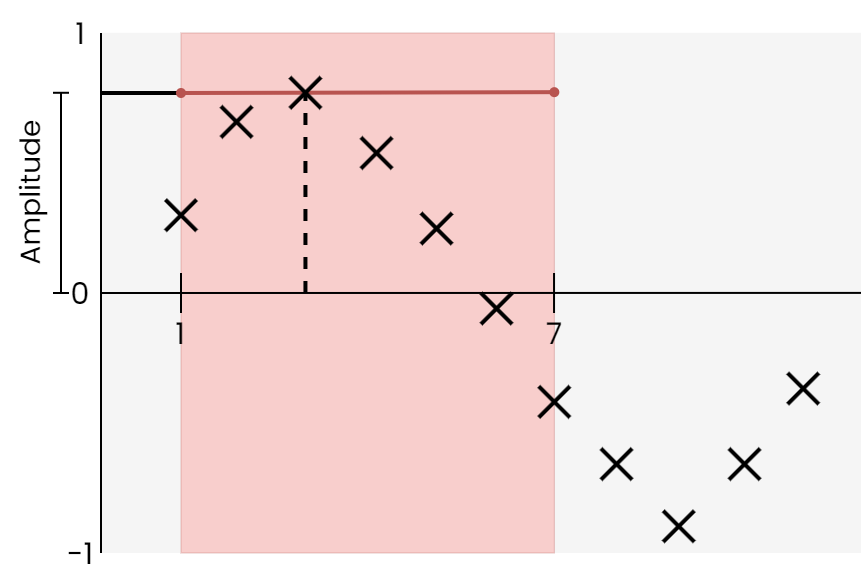
\includegraphics[scale=0.3]{images/amplitude_example.png}
    \caption{This diagram illustrates how we get the amplitude of an audio clip within a given range. Here the range is [1,7] and the sample with the highest absolute magnitude is the 3rd.}
    \label{fig:amplitude}
\end{figure}

In order to generate a waveform overview, the audio needs to be split into a set of ranges and the amplitude of each range found. In tuPAC, this is done with \Fref[main]{alg:waveform}. For a given bounding box, this algorithm generates an array of bar heights corresponding to a given audio file. This waveform can then be drawn as a collection of vertical lines in the \sample's \verb|draw| function.

\begin{figure}[h]
    \centering
    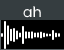
\includegraphics[scale=1.5]{images/sample.png}
    \caption{Example of a waveform drawn on a \sample.}
    \label{fig:my_label}
\end{figure}

\begin{algorithm}[H]
\DontPrintSemicolon
\SetKwInput{Input}{Input}\SetKwInOut{Data}{Constants}
\Input{\textit{WaveformLength}: In pixels, the horizontal length of the waveform.
\newline
\textit{WaveformHeight}: In pixels, the maximum vertical height of bars in the waveform.
\newline
\textit{ArrayOfSamples}: The buffer from Tone.js, arbitrarily large.}
\Data{\textit{BarThickness}: In pixels, the thickness of each bar when drawn.
\newline
\textit{BarPad}: In pixels, the distance between bars when drawn.
\newline
\textit{MaxWidth}: In samples, the maximum size of the range to get amplitude from.}
\vspace{1mm} \hrule \vspace{1mm}
\nl $NumberOfBars \gets WaveformLength/(BarThickness + BarPad)$\;
\nl $Waveform \gets []$\;
\nl $Ratio \gets ArrayOfSamples.length / NumberOfBars$\;
\nl $Width \gets \lfloor min(MaxWidth, ratio)/2\rfloor$\;
\nl \For{$i=0$ to $bars-1$}{
    \nl $Centre \gets i * Ratio$\;
    \nl $Range \gets [Centre-Width, Centre+Width]$\;
    \nl $Waveform[i] \gets max_{j\in Range}(|j|)$\;
}
\nl $MaxValue \gets max_{n\in Waveform}(n)$\;
\nl \For{$i=0$ to $bars-1$}{
    \nl $Waveform[i] \gets WaveformHeight * Waveform[i] / Max$\;
}
\caption{tuPAC waveform generation algorithm}\label{alg:waveform}
\end{algorithm}

ADD COMMENTS TO ALGORITHM

In tuPAC, the audio generation is done with Tone.js. After loading a sound file to be played in a \sample\ we can acquire an array for floating point numbers between -1 and 1 representing the magnitude of each sample in the audio file. We can then run \Fref[main]{alg:waveform} on this array to get an array of bar heights.

When we generate the waveform, we are generating an array of arbitrary size from an array of arbitrary size. Thus, we must ensure that no matter what size each array is we will get a waveform that approximately represents the audio.

\begin{figure}
\centering
\begin{subfigure}{.5\textwidth}
  \centering
  \includegraphics[width=.4\linewidth]{image1}
  \caption{A subfigure}
  \label{fig:sub1}
\end{subfigure}%
\begin{subfigure}{.5\textwidth}
  \centering
  \includegraphics[width=.4\linewidth]{image1}
  \caption{A subfigure}
  \label{fig:sub2}
\end{subfigure}
\caption{A figure with two subfigures}
\label{fig:test}
\end{figure}

\begin{figure}
    \centering
    \includegraphics{}
    \caption{Caption}
    \label{fig:my_label}
\end{figure}

\subsection{Time Bar Translation}\label{sec:timebar_translate}
A feature that was wanted for tuPAC was to allow \canvas es to run at different speeds. However, this results in \timebar s moving at different speeds, which could be visually confusing and difficult to understand for the user. To solve this, there is a space in which the \timebar\ of a child \canvas\ has a line connecting it to the parent \canvas's \timebar, as shown in \Fref[main]{fig:timebartranslation}.

\begin{figure}[h]
    \centering
    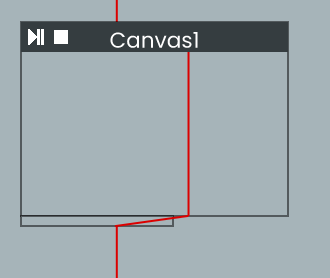
\includegraphics{images/timebartranslate.png}
    \caption{Example of a \timebar\ being ``translated".}
    \label{fig:timebartranslation}
\end{figure}

This feature is essential to helping users see how \canvas es work (maybe cite evaluation here) but it also serves a functional purpose. Naturally, as this box translates between the speeds of the two \canvas es, it's horizontal size represents the duration of the child \canvas, at the parent \canvas' speed. When resized, the child \canvas' speed changes to represent the box's size. This means that the \canvas' playback last exactly during the time the parent \timebar\ is over this translation box.

\subsection{Effects}
The \effect\ class provides a way of applying distortion or reverb to the sounds in tuPAC. As shown in \Fref[main]{fig:element_inheritance}, it extends the same class as \canvas, allowing for other \playable s to be held by an \effect. \effect s, however, can only hold one \element\ and it cannot be moved around. In order to do this, a \canvas could instead be put into an \effect\ instead.


\subsection{Rendering}
\subsection{Playback}
In tuPAC, all \element s have a horizontal size which directly correlates to their length in time when playing back. With \canvas es this can be manipulated as described in \Fref[main]{sec:timebar_translate}, but it is imperative that this length always correlates to the duration of playback. As mentioned previously all playback is done with Tone.js. 

\subsection{Repository overview}
In summary, I present an overview of the file structure of the project. All code in the \verb|src| directory was written from scratch after the research and preparation phases of the project were complete and the framework for the software was decided. The other code (the contents of \verb|main.js|, \verb|index.html|, \verb|jest.config.js| and \verb|tsconfig.json|) was written with the help of online guides, as they are more generic files pertaining to Electron, Jest and TypeScript. All images used in the program are in \verb|resource/img/| and were created by me from scratch. The font stored in \verb|resource/font/| was taken from Google Fonts, under the Open Font License.

\DTsetlength{0.2em}{1em}{0.2em}{0.4pt}{2pt}
\setlength{\DTbaselineskip}{20pt}
\dirtree{%
.1 .
.1 dist/\DTcomment{The files to be run by Electron (Compiled JS files and HTML)}.
.2 index.html\DTcomment{The webpage that renders in Electron}.
.1 resource/\DTcomment{Resources other than code needed for the software}.
.2 img/.
.2 font/.
.1 src/\DTcomment{The source TypeScript files to be compiled}.
.2 capsule.ts.
.2 canvas.ts.
.2 ....
.2 tupac.ts\DTcomment{The code run in index.html to render the GUI}.
.1 test/\DTcomment{Unit tests to be run with Jest}.
.1 main.js\DTcomment{The initial code run, which opens the Electron window}.
.1 jest.config.js\DTcomment{Configuration for Jest testing}.
.1 tsconfig.json\DTcomment{Configuration for TypeScript compilation}.
}

The repository consists mainly of two folders. \verb|src| contains the TypeScript files which compile into \verb|dist|, which contains the files used at runtime. \verb|dist| also contains the HMTL file which is displayed when Electron runs. The TypeScript files compile to CommonJS modules, which are imported and used by the other files. For example, the file \verb|tupac.ts| imports the module ``window", which after compilation is done by importing the \verb|window.js| file.

\chapter{Evaluation}
As mentioned in the preparation chapter, the success of this project leans on the successful implementation of a set of features, and the extent to which it enables artists to easily create phonological compositions. The latter is infeasible to directly evaluate, as it would be extremely difficult to find a large sample of people interested in this style of composition who would be willing to participate in a study. Instead, I chose to do general user testing on the usability and clarity of the program, which indicates the efficacy of the design and implementation of the project.

\section{Functionality}

\subsection{Unit Testing}

\section{User Testing}

\subsection{}


\chapter{Conclusions}
\section{Project Summary}
The project was successful. A novel system was designed and developed which provides an alternative to modern composition techniques which improves the digital composition process for particular styles of composition, particularly those which utilise the layering, repetition and augmentation of parts of speech. The functionality and design of the system were decided with input from an artist interested in phonological composition and the final result accurately reflected what they wanted from such a system.

\section{Further Work}
The system that has been developed is somewhat lacking in features due to the limited scope of the project and difficulty of certain desired functionality. This project has provided the theoretical and practical basis for further exploration into the potential of audio composition interfaces and their ability to assist in the creation of music.

%TC:ignore
%%%%%%%%%%%%%%%%%%%%%%%%%%%%%%%%%%%%%%%%%%%%%%%%%%%%%%%%%%%%%%%%%%%%%
% the bibliography
\addcontentsline{toc}{chapter}{Bibliography}
\bibliography{refs}

%%%%%%%%%%%%%%%%%%%%%%%%%%%%%%%%%%%%%%%%%%%%%%%%%%%%%%%%%%%%%%%%%%%%%
% the appendices
\appendix

\chapter{Latex source}

\section{metadata.tex}
{\scriptsize\verbatiminput{metadata.tex}}

\section{main.tex}
{\scriptsize\verbatiminput{main.tex}}

\section{proposal.tex}
{\scriptsize\verbatiminput{proposal.tex}}

\chapter{Makefile}

\section{makefile}\label{makefile}
{\scriptsize\verbatiminput{makefile.txt}}

\section{refs.bib}
{\scriptsize\verbatiminput{refs.bib}}


\chapter{Project Proposal}

\documentclass{article}
\usepackage[utf8]{inputenc}
\usepackage{graphicx}
\usepackage[indent=0pt,skip=10pt]{parskip}
\usepackage[a4paper, total={6in,8in}]{geometry}

\begin{document}

\section*{Introduction}

There exists a wide variety of digital tools to aid the composition of music. Modern DAWs (Digital Audio Workstations) such as Ableton and Fruity Loops are used extensively in the recording, mixing and mastering of most of the music that is produced today. These applications are designed to allow musicians to easily rearrange, layer and manipulate snippets of audio which can be imported from external sources, recorded onto the tracks or generated by MIDI instruments. While this design makes musical composition and recording simple and accessible for many popular styles of music, it can be restricting to other styles of composition and inhibit explorations into more niche musical expressions. 
\begin{figure}[h]
    \centering
    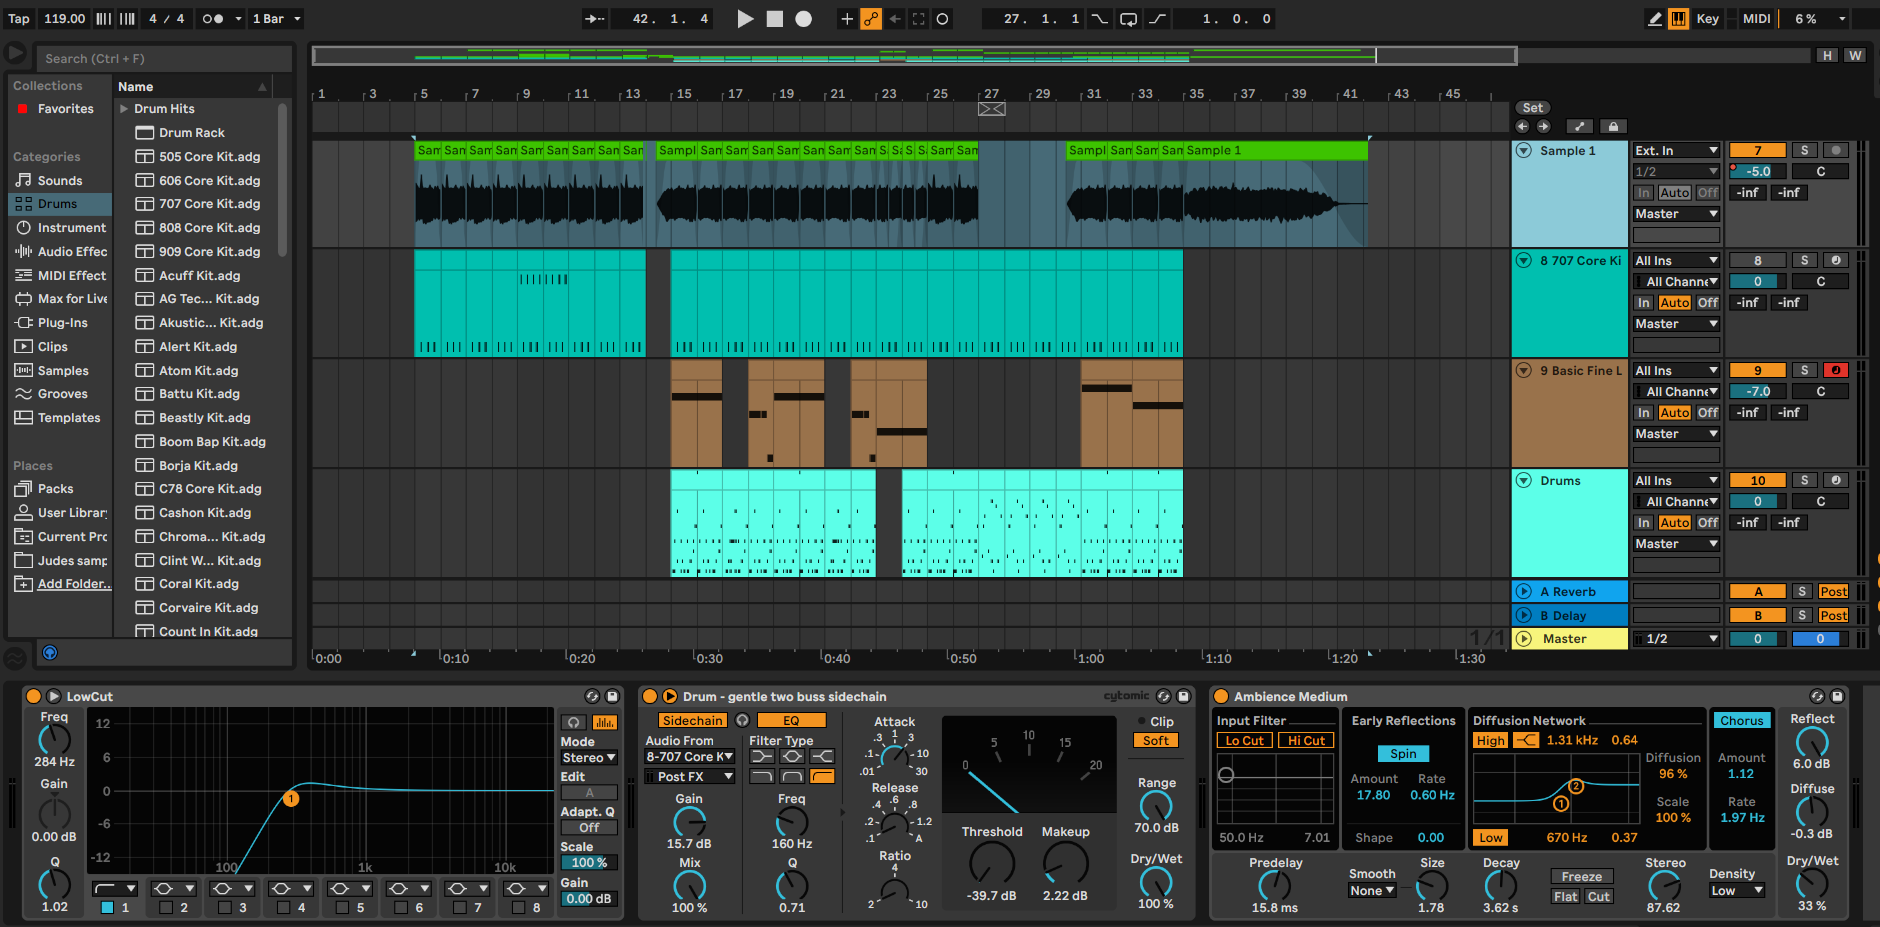
\includegraphics[scale=0.3]{images/ableton example.png}
    \caption{An example of an industry-standard DAW (Ableton 11)}
    \label{fig:ableton}
\end{figure}

Another style of digital music composition that is particularly relevant to my project is through live coding techniques. Live coding (with regards to musical composition) is a performance art in which the artist types code in front of an audience, into an environment which translates the code into music.

TidalCycles is one such platform. Tidal is software which allows people to create music through programming. Users create rhythmic patterns and generate sounds from synths or play samples as dictated by these patterns. It is embedded in the Haskell programming language and uses a custom synth and sampler called SuperDirt, built on the SuperCollider platform.

For my project, I will create an interactive music composition tool which facilitates the composition of music using speech sounds. These sounds may be generated digitally or from small samples of real recordings. I will build a text-based tool on top of an existing text-based audio generation platform (Strudel or Sonic Pi) which will allow users to create music from small literals representing snippets of speech, as well as a graphical user interface which allows users to rearrange and connect blocks to generate audio, in a style similar to the popular visual programming language Scratch.

Strudel is a web-based live coding environment intended to replicate the ideas of TidalCycles, but instead built on JavaScript and run in a browser. It uses a few different browser-available playback methods, most notably the Web Audio API and Tone.JS. There is a work-in-progress feature which allows it to communicate with SuperCollider and run SuperDirt.
\begin{figure}[ht]
    \centering
    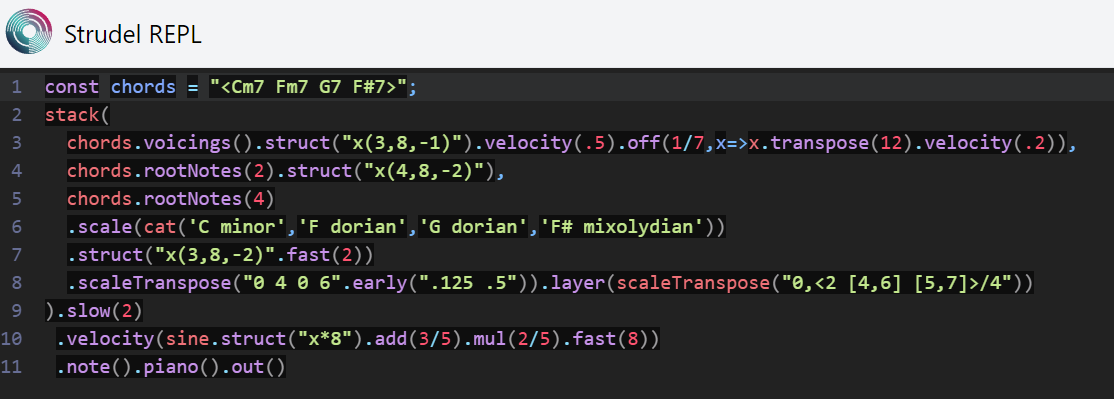
\includegraphics[scale=0.5]{images/strudel.png}
    \caption{The Strudel REPL (web-based application which runs Strudel), with example code/music}
    \label{fig:strudel}
\end{figure}

Another example of a live coding platform that I could work with is Sonic Pi, which is a standalone application with a much simpler language to write music and more in-depth tools than Strudel, but it is more limiting in the ease of expressiveness of the language. It is written in C++ and Ruby. It also uses SuperCollider to generate audio.
\section*{Starting Point}
I have very little experience with live coding and digital audio generation. I have no experience working in JavaScript or Ruby. I will need to learn about how Strudel and Sonic Pi work during the project, and will need to learn how to work with JavaScript or Ruby.
\section*{Substance of Project}
\subsection*{Core}
I will produce a piece of software which allows users to write code and generate audio from speech sounds in order to create music. Users will be able to take small snippets of speech and combine them by playing them back in a chosen order, with a chosen rhythm, by layering them, and by manipulating them in various ways.

I will also produce a piece of software which allows user to achieve a similar goal through diagrammatic means. A GUI will allow a user to take small speech literals as blocks and order them, pass them through filters, layer them or loop them.

Although tools exist that already allow you to do what my project will achieve, it will greatly improve the efficiency for a style of composition which, to my knowledge, has no tools dedicated to enabling it. You can achieve what my project will achieve in a standard DAW, but my tool will allow users to achieve more complicated rhythms and structures in much less time than they would moving samples of speech around in a DAW. It also makes the process much more accessible, allowing users with little experience working with digital composition tools or with programming to work with this style of proposition and to work with live coding techniques.
\subsection*{Extensions}
Some possibles extensions of my project would:
\begin{itemize}
    \item Build an explicit formal language describing the composition and generation of audio, based on the text-based tool.
    \item Change the text-based tool to reflect the definition of the formal language.
    \item Change the graphical tool to represent this formal language.
    \item Integrate neural synthesis of speech sounds into my composition tool. Antoine Caillon and Philippe Esling released a paper last year detailing a variational auto-encoder they have developed (RAVE) which allows for fast, high quality audio synthesis. I could implement RAVE into the tool to allow users to generate their own speech audio with state-of-the-art neural synthesis, adjusting parameters to change the sound in real time.
\end{itemize}
\section*{Success Criterion}
In order to have succeeded in my project, I require:
\begin{itemize}
    \item Software which allows users to write code which will use speech sounds to generate an audio output.
    \item Software which allows users to rearrange blocks specifying speech sounds and operations on those sounds in order to generate an audio output.
    \item Both pieces of software should allow for users to:
    \begin{itemize}
        \item Play back a small sample of speech.
        \item Arrange multiple sounds to be played back with a particular rhythm and order.
        \item Layer multiple sounds to be played alongside each other.
        \item Manipulate sounds with filters and effects.
    \end{itemize}
    \item The software be evaluated against an industry-standard DAW in user tests to express the efficacy of both the graphical and text-based tool in the production of phonological music.
\end{itemize}
For the final bullet point, I will supply the software to users who will give written feedback on the ease of use of my tool and existing tools. I will also measure the time taken for users to complete specific tasks to measure quantitatively the improvement on certain tasks over existing tools. I will use A/B testing to compare the two implementations, text-based and graphical, to measure the ease of use for each tool.
\section*{Timetable}
\subsection*{Feedback}
Over the duration of my project, I plan to interact with users for feedback. I am already in contact with one artist and I will venture to find other possible users of my tool through people I know and get feedback from a wider source. In the first few weeks, I will need to fill in the form for the Ethics Committee to approve the involvement of human participants.
\subsection*{Week 1/2: 16th Oct. - 29th Oct.}
\begin{itemize}
    \item Study Strudel framework.
    \item Study Sonic Pi framework.
    \item Set up work environment for development of text-based tool.
\end{itemize}
{
\centering\textbf{Milestone:} Decide whether to work with Strudel or Sonic Pi, supplying a report describing the details of the research and my choice to my supervisor. Be able to compile and run Strudel and/or Sonic Pi on my own machine, allowing for my own modifications and additions to the code.
}
\subsection*{Week 3/4: 30th Oct. - 12th Nov.}
\begin{itemize}
    \item Research system for generation of audio.
    \item Understand how to generate, combine and manipulate audio to produce new outputs.
\end{itemize}
{
\centering\textbf{Milestone:} Write program which is able to generate sample audio outputs, working on samples given by user.
}
\subsection*{Week 5/6: 13th Nov. - 26th Nov.}
\begin{itemize}
    \item Begin programming of text-based composition tool.
\end{itemize}
{
\centering\textbf{Milestone:} Have functioning text-based tool which allows users to input code and generate audio using small snippets of speech.
}
\subsection*{Week 7/8: 27th Nov. - 10th Dec.}
\textit{Michaelmas term ends: 1st Dec. Varsity skiing trip}
\begin{itemize}
    \item Continue work on text-based tool.
    \item Test text-based implementation on user, get feedback.
\end{itemize}
{
\centering\textbf{Milestone:} Report describing user feedback, possible improvements and tweaks to system.
}
\subsection*{Week 9/10: 11th Dec. - 24th Dec.}
\begin{itemize}
    \item Refine text-based tool based on feedback.
\end{itemize}
{
\centering\textbf{Milestone:} New, improved version of tool modified based on the feedback from the user.
}
\subsection*{Week 11/12: 25th Dec. - 7th Jan.}
\textit{Christmas and New Years Eve, will not be completing much work.}
\begin{itemize}
    \item Research libraries for creating visual programming languages (e.g. Blockly).
\end{itemize}
{
\centering\textbf{Milestone:} Write up a page for project supervisor describing what I have learnt, what library I will use and how I will use the library to create a GUI.
}
\subsection*{Week 13/14: 8th Jan. - 21st Jan.}
\textit{Lent term starts: 17th Jan.}
\begin{itemize}
    \item Build diagrammatic tool for phonological audio composition.
\end{itemize}
{
\centering\textbf{Milestone:} Working GUI, allowing users to rearrange blocks in order to generate audio in different ways.
}
\subsection*{Week 15/16: 22nd Jan. - 4th Feb.}
\textit{Progress deadline due: 3rd Feb (12pm)}
\begin{itemize}
    \item Feedback from user.
    \item Improve on GUI.
    \item Write progress report.
\end{itemize}
{
\centering\textbf{Milestone:} Hand-in progress report, written evaluation of user feedback.
}
\subsection*{Week 17/18: 5th Feb. - 18th Feb.}
\begin{itemize}
    \item Start writing the dissertation.
\end{itemize}
{
\centering\textbf{Milestone:} Complete draft chapter to be reviewed by project supervisor.
}
\subsection*{Week 19/20: 19th Feb. - 4th Mar.}
\textit{Slack: time for me to catch up if running behind, complete extensions if ahead.}
\subsection*{Week 21/22: 5th Mar. - 18th Mar.}
Continue to write dissertation.

{
\centering\textbf{Milestone:} Draft of Introduction, Preparation chapters to be sent to supervisor.
}
\subsection*{Week 23/24: 19th Mar. - 1st Apr.}
Continue to write dissertation.
{

\centering\textbf{Milestone:} Draft of Implementation, Evaluation chapters to be sent to supervisor.
}
\subsection*{Week 25/26: 2nd Apr. - 15th Apr.}
Continue to write dissertation.

{
\centering\textbf{Milestone:} Full draft of dissertation to be sent to supervisor.
}
\subsection*{Week 27/28: 16th Apr. - 29th Apr.}
\textit{Slack: time for me to push back goals into.}
\subsection*{Week 29/30: 30th Apr. - 12th May}
\begin{itemize}
    \item Final touch-ups.
    \item Hand in final dissertation.
\end{itemize}
{
\centering\textbf{Milestone:} Finish project!
}

\textit{Note: During the weeks of writing the dissertation, I will periodically be sending the drafts to my supervisor for feedback, and improving on them when feedback is received.}
\section*{Resource Declaration}
My own laptop is sufficient to complete this project. No particularly heavy computation will be necessary. I don't have much storage left on my laptop, so I will need to acquire an extra SSD. The software and libraries that I will be using in this project is all publicly available (Strudel, Blockly, Sonic Pi, SuperDirt,  etc.). I will use a GitHub repository to store my code as well as my own laptop storage, and so in case of a failure of my laptop I will have a back-up of my work.
\textit{I accept full responsibility for this machine and I have made contingency plans to protect myself against hardware and/or software failure.}
\end{document}

%TC:endignore
\end{document}